% !TEX root = ../22830110_dissertation.tex
\chapter{Analysis and Design of the Proposed Solution}
\label{chap:analysis_design}

\section{System Requirements and Constraints}
Developing software for financial compliance introduces exceptionally rigorous constraints. A single rounding error or unverified assumption can invalidate an entire financial report. The analysis phase identified three primary layers required for the architecture:
\begin{enumerate}
    \item \textbf{Ingestion (ETL) Layer:} Securely handling Xero OAuth2 authentication, extracting transactional data, and normalising it into a deterministic format.
    \item \textbf{Rules Engine (Core Layer):} A deterministic mathematical engine. This layer computes variances and Prior-Year (PY) comparisons. It enforces the ``Decimal Mandate,'' strictly prohibiting \texttt{float} data types in favor of \texttt{decimal.Decimal} with \texttt{ROUND\_HALF\_UP}. It also integrates robust statistical analysis on historical transactions to identify material drivers, recurring subscriptions, and potential anomalies prior to the synthesis phase.
    \item \textbf{Synthesis (NLG Layer):} The Natural Language Generation layer, responsible for translating the deterministic numeric outputs into human-readable, professional narrative.
\end{enumerate}

\section{Firm-Standard Variance Logic and Triggers}
The system design incorporates specific materiality thresholds. The AI must flag and generate commentary for variances greater than 10\%. Trivial changes are filtered out, except for ``Mandatory Comment Accounts'' which require commentary regardless of variance magnitude. These include Directors' Remuneration, Legal \& Professional Fees, Donations \& Entertainment, and Bad Debts.

\section{Security, Privacy, and Anonymisation}
Because the system handles sensitive financial data, compliance with UK GDPR is a basic requirement. The design follows the core principles highlighted in the UK Information Commissioner's Office (ICO) guidance: purpose limitation, data minimisation, storage limitation, integrity/confidentiality, and accountability (\url{https://ico.org.uk/for-organisations/uk-gdpr-guidance-and-resources/data-protection-principles/a-guide-to-the-data-protection-principles/}). The system is framed as a draft-generation tool for year-end working papers only; it is not a general-purpose document store or autonomous filing agent.

An Anonymisation Layer (DataMasker) was designed to redact Personally Identifiable Information (PII) such as director names, sensitive supplier names, personal addresses, and free-text references that could expose natural persons. This reflects the ICO's data-minimisation expectation that organisations should process only data that is adequate, relevant, and limited to what is necessary for the stated purpose (\url{https://ico.org.uk/for-organisations/uk-gdpr-guidance-and-resources/data-protection-principles/a-guide-to-the-data-protection-principles/data-minimisation/}). Where redaction would materially damage accounting meaning, the design instead prefers pseudonymisation and controlled access for authorised reviewers.

The system also raises specific privacy concerns in a professional-services context:
\begin{itemize}
    \item \textbf{Director and employee data:} payroll narratives, directors' loan accounts, and benefits-in-kind commentary may expose personal financial behaviour.
    \item \textbf{Supplier and customer identification:} one-off payees, legal advisers, and related-party entities may reveal commercially sensitive relationships.
    \item \textbf{Retention risk:} prompts, completions, and exported logs must not be kept indefinitely once the review cycle is complete, in line with the storage-limitation principle (\url{https://ico.org.uk/for-organisations/uk-gdpr-guidance-and-resources/data-protection-principles/a-guide-to-the-data-protection-principles/storage-limitation/}).
    \item \textbf{Human oversight:} because generated notes may contain hallucinated or misattributed commentary, a qualified accountant remains accountable for final review before any client-facing use.
\end{itemize}

\begin{figure}[H]
    \centering
    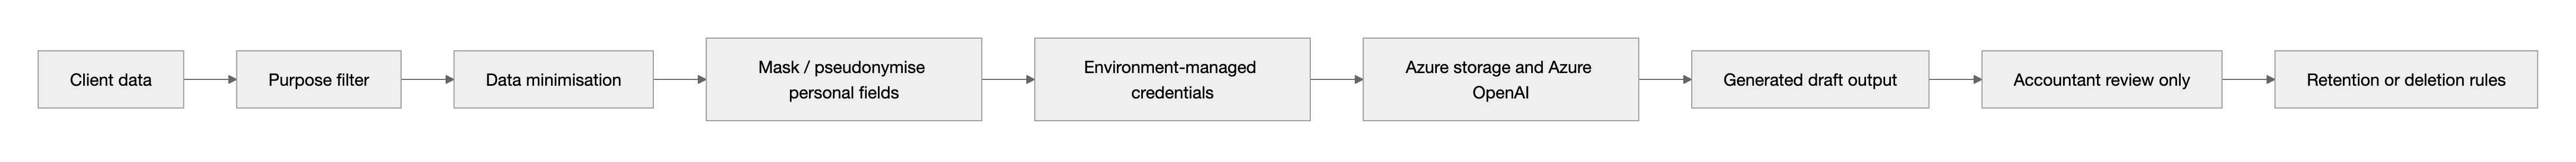
\includegraphics[width=0.72\textwidth]{figures/privacy_controls_flow}
    \caption{Privacy and Control Gates Applied to Client Data Before and After Generation}
    \label{fig:privacy_controls_flow}
\end{figure}

Figure \ref{fig:privacy_controls_flow} summarises the control path assumed in the design. The main point is that the model should not be treated as the first place where privacy is considered. Purpose filtering, minimisation, masking, credential handling, accountant-only review, and retention controls all sit around the generation step.

The cloud deployment choice was also influenced by provider privacy controls. Microsoft states that prompts, completions, and fine-tuning data sent to Azure OpenAI are not shared with other customers, are not available to OpenAI, and are not used to train or improve the foundation models (\url{https://learn.microsoft.com/en-us/legal/cognitive-services/openai/data-privacy}). This does not remove the need for local controls, but it does make the Azure-hosted deployment materially more appropriate than consumer-grade tooling for professional accounting data. In other words, Azure was chosen not merely for convenience, but because the project required a platform with enterprise data-protection guarantees that were more compatible with handling confidential company working-paper material.

This security posture also affects what can be submitted publicly. The dissertation repository includes the code required to reproduce the pipeline and evaluation workflow, but it does not include live \texttt{.env} credential files or active service secrets. Those values provide access to protected company-connected resources and therefore fall outside the scope of safe academic submission. A supervised live demonstration of the system is instead available on request.

\section{Interface and User Experience Design}
The design of the application's interface was governed by the requirement for "Clarity over Decoration." Financial professionals require a tool that minimizes cognitive load while maximizing data visibility. 

The user interface was designed with a "Side-by-Side Review" paradigm. This allows the user to see the raw financial data on the left and the AI-generated narrative on the right, facilitating immediate verification. The interface also incorporates "Confidence Scoring" and "Provenance Tracking," where specific numeric values in the narrative are linked back to their source ledger entries, creating a transparent and audit-ready review environment.

\subsection{Wireframe Architecture and User Journey}
The design phase involved the creation of low-fidelity and high-fidelity wireframes to map the accountant's workflow. This journey was segmented into three primary stages:
\begin{enumerate}
    \item \textbf{Secure Ingress:} A streamlined authentication interface designed to emphasize data security from the first interaction.
    \item \textbf{Client Monitoring Workbench:} A data-dense dashboard providing a high-level overview of the entire client portfolio, enabling accountants to manage multiple review cycles simultaneously without navigational friction.
    \item \textbf{The Synthesis Hub:} The primary interaction point where the "Side-by-Side Review" logic is implemented. This hub allows users to provide direct feedback to the AI for narrative regeneration, bridging the gap between automated drafting and human professional judgement.
\end{enumerate}
